% Chapter 6

\chapter{Case studies and results} % Main chapter title

\label{results} % For referencing the chapter elsewhere, use \ref{Chapter1} 

\lhead{Chapter 6. \emph{Results and Discussion}} % This is for the header on each page - perhaps a shortened title

%----------------------------------------------------------------------------------------

This chapter will present the cases investigated and the results achieved.
The main tools in addition to Nek5000 needed to perform the simulations presented in this 
chapter are \textit{ANSYS ICEM} and \textit{python}. For post-processing \textit{Visit} and
\textit{Matlab} were used.
%
\section{Case 1: Gas dispersion in a simplified urban area}
%The problem investigated in this work is gas dispersion of neutral gas in a velocity field through four cubic blocks.
%Similar simulations have been done in CDP and Fluent which are compared to data from a wind-tunnel experiment performed by ALAN.
The scenario investigated in this work is dispersion of a neutral gas in a rectangular tunnel
with four cubic blocks placed as obstacles. The blocks have sides $h = 0.109$m and represent a 
set of buildings forming a street canyon. The gas is released from a circular source on 
ground level and
is translated by the wind field through the canyon, see \fref{fig:layout}.
In this figure $h$ have been used as the length scale. The dotted lines
indicate the positions where data is collected.
%
\begin{figure}[h]
	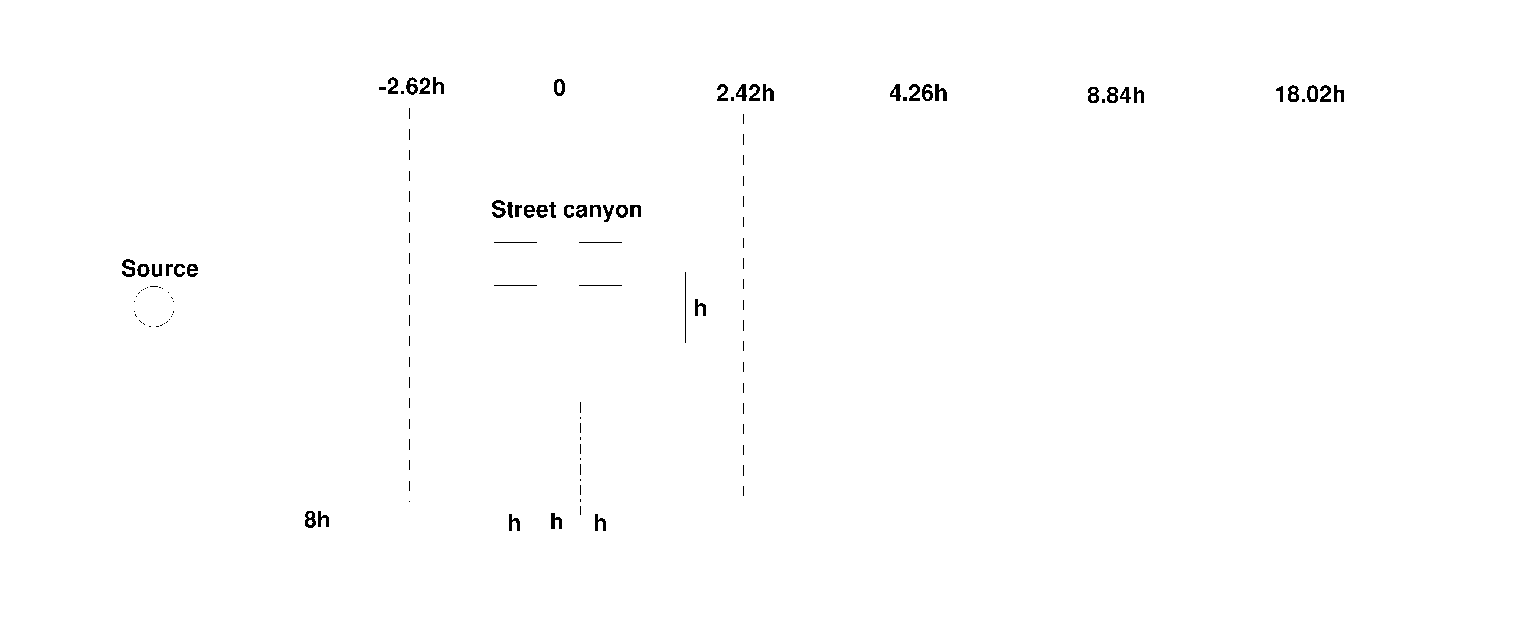
\includegraphics[width=1.1\textwidth]{Figures/layout.eps}
	\caption{Schematic overview of the domain from above. The data is collected along the dotted lines.}
	\label{fig:layout}
\end{figure}
%

Scaling the domain with the size of the boundary layer $H =1$m restricts it to
the box $0.0\leq x/H \leq 4.96,-1.75\leq y/H \leq 1.75, 0\leq z/H \leq 1.5$.
The four cubic boxes are centered around $(1.4315,0)$ with a distance $h$ between each box.
The source is placed with its center in $(0.396,0)$ and radius $r = 0.0515$.
The grid used for the computations consists of 14747 elements and with a polynomial degree of
8 the total number of nodes $N\approx 7,6$mill. 


The simulations are performed using Large Eddy Simulation (LES) 
with the dynamic Smagorinsky-Lilly subgrid-scale model and by applying the polynomial filtering
routine that is available in Nek5000. 
The release of gas will result in a plume that is advected with the wind field,
see \fref{fig:plume}. The concentration of the released gas at the 
indicated positions in \fref{fig:layout} are compared with 
experimental data and simulations performed in CDP~\cite{CDP}. 
For clarification some of the variables repeatedly mentioned throughout this thesis will be 
stated explicitly in \tref{tab:simplevariables}.
\begin{table}
    \centering
    \begin{tabular}{c c c c}
        Variable & value & unit & commentary \\ \hline
        $H$   & $1$ & m & length scale of the domain \\ 
        $h$   & $0.109$ & m & the sides of the cubic boxes\\ 
        $Q$   & $50$ & dm$^3$/min & gas release from source \\ 
        $U_{ref} $& $\approx1.08$ & m/s & reference value of $U$ \\
    \end{tabular}
    \caption{Essential variables, $U_{ref}$ is calculated as a time average of the velocity in 
        x-direction at a point far away from the floor and walls and will therefore 
        vary by a small amount from case to case. }
    \label{tab:simplevariables}
\end{table}

The inflow conditions had to be extrapolated onto the domain at each time step. To mimic the situation in the wind-tunnel the velocity field
on the inflow was generated in a different simulation performed in CDP. The inflow velocity was written to file every 
$0.0013$s for a total of $28$s and had to be interpolated onto the domain for the simulations in Nek5000 since the grid was not identical.
The right plot in \fref{fig:inflow} is an instantaneous picture of the inflow velocity in x-direction, 
notice how the pattern repeats itself along the y-axis. This is because the inflow data was generated in a smaller channel, approximately $1/3$ of the 
width of the computational domain used for the data sampling. An interpolation algorithm implemented at FFI was applied in order to adjust 
the inflow-data to the computational mesh, this was done directly in \verb|.usr|. 
%
\begin{figure}
\centering
  \centerline{
\begin{minipage}{.6\textwidth}
  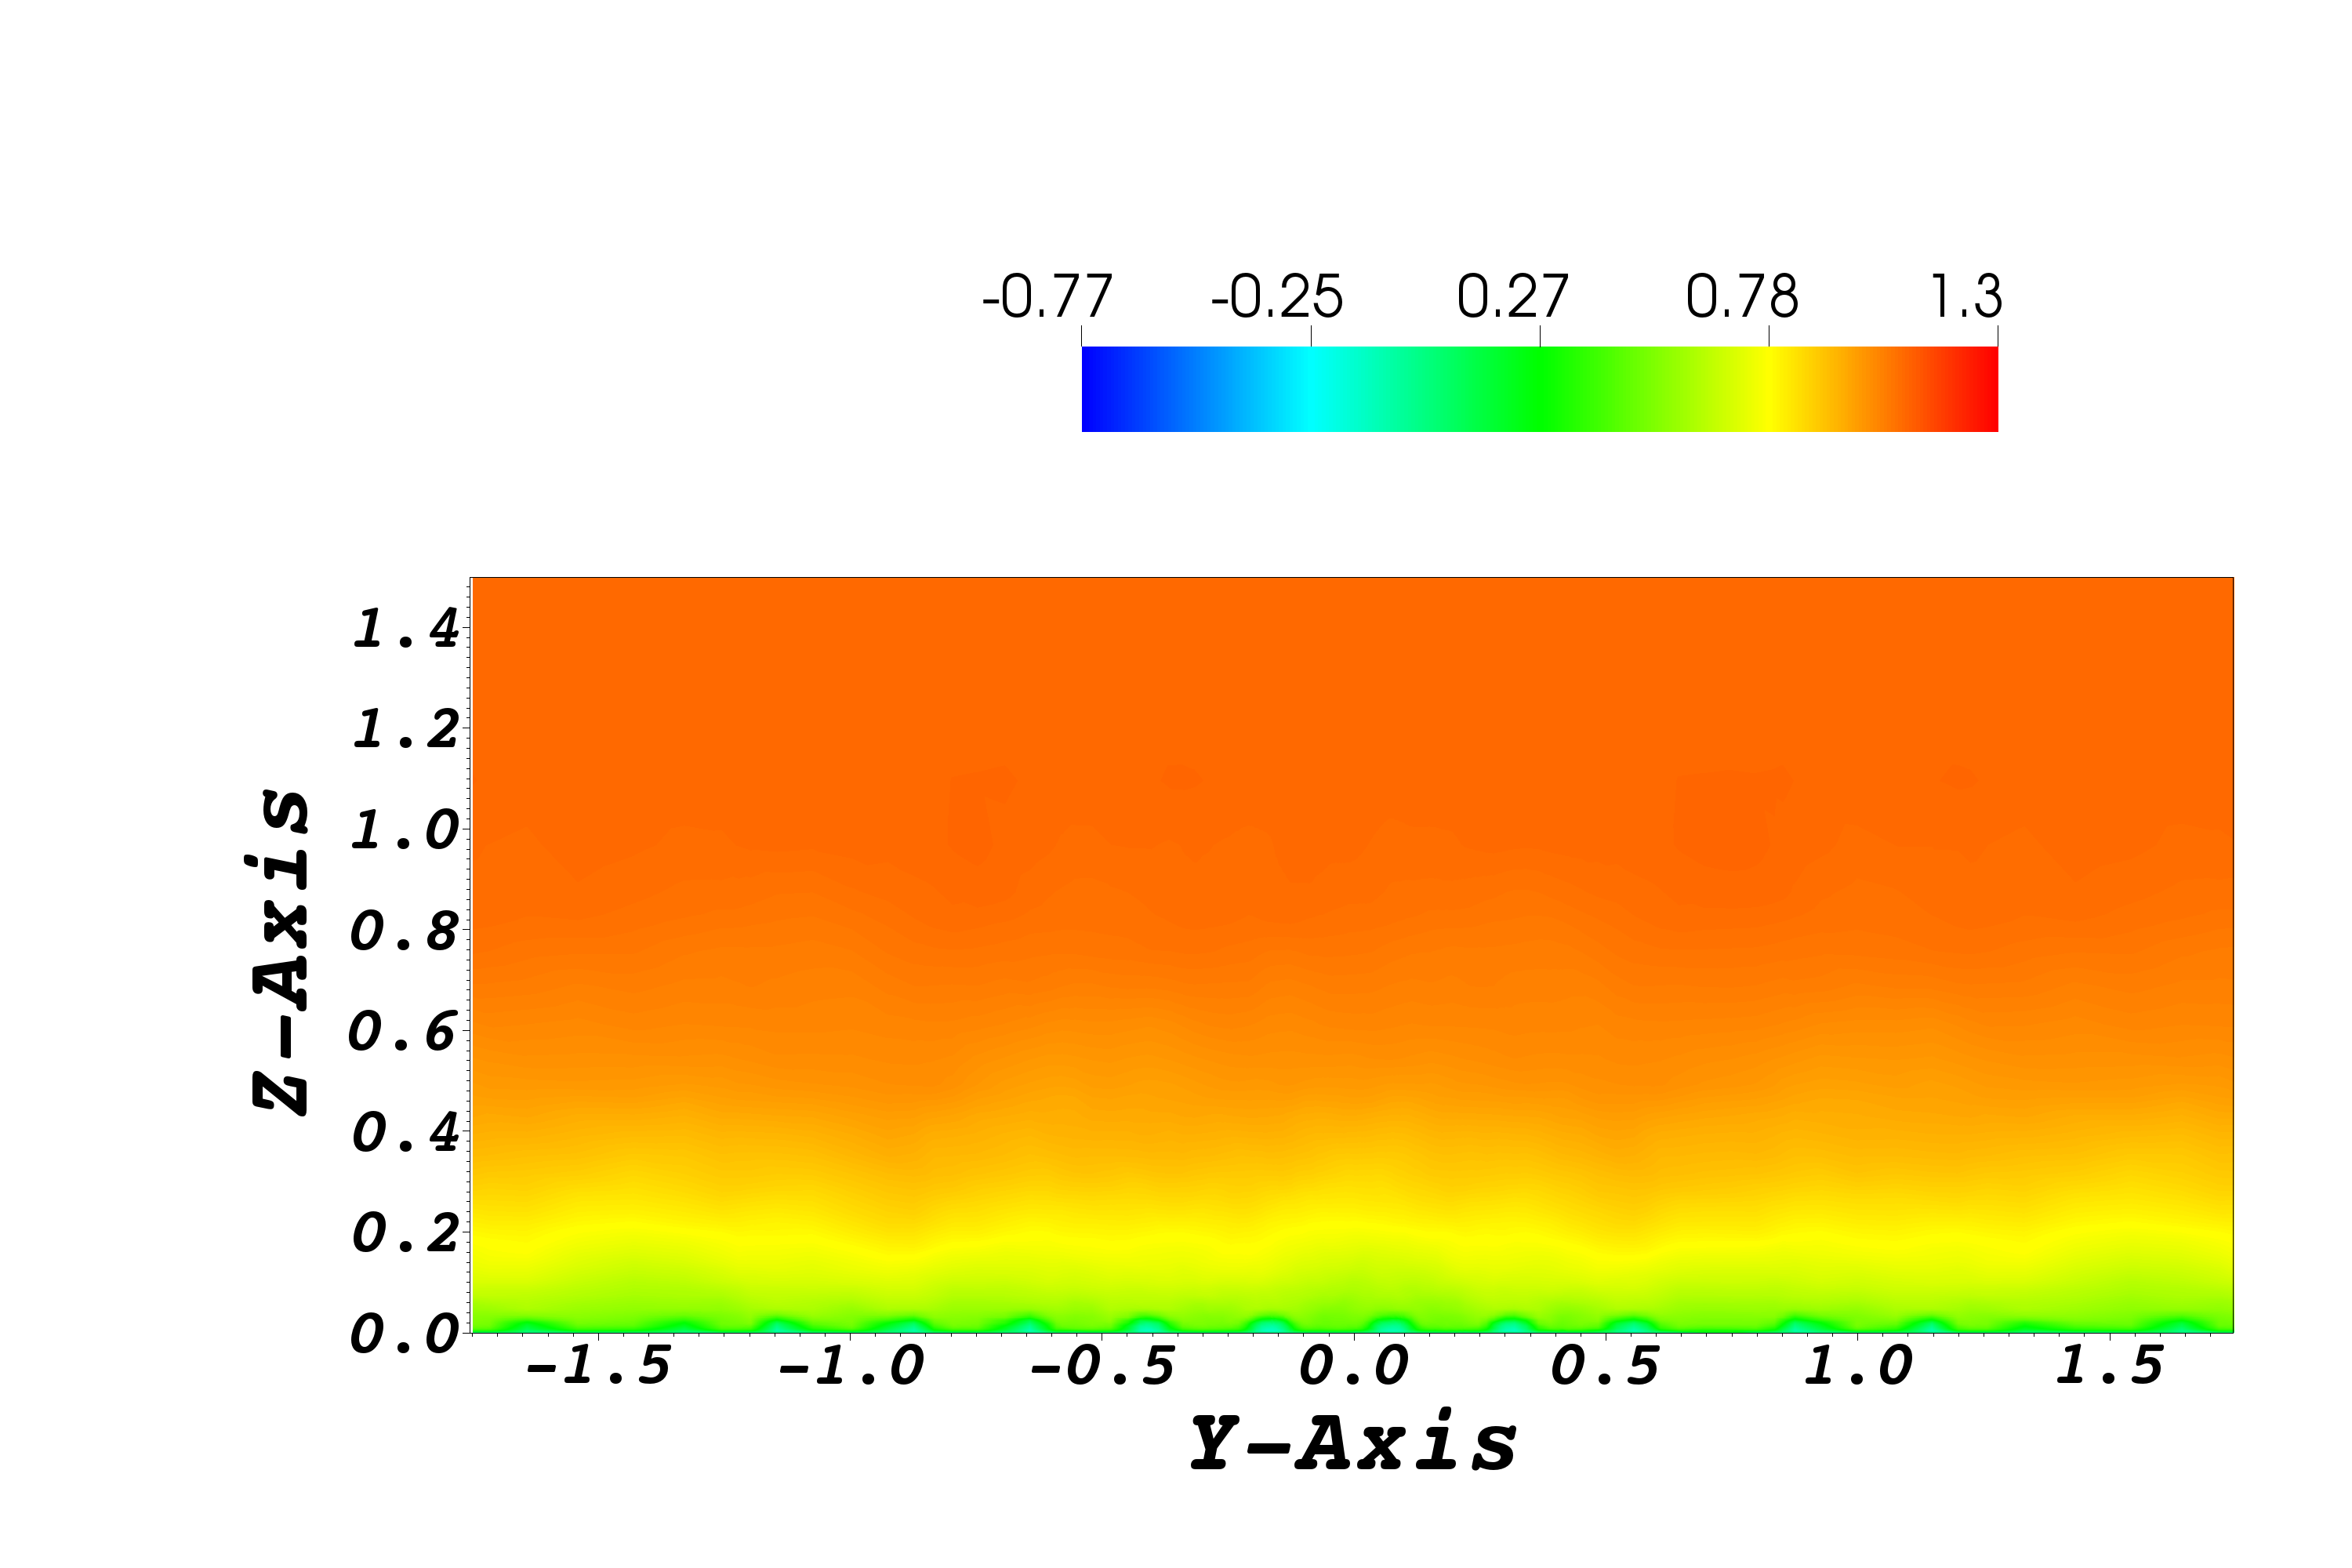
\includegraphics[width=1.0\linewidth]{Figures/inflow_field_avg.png}
  %\captionof{figure}{A figure}
\end{minipage}%
\begin{minipage}{.6\textwidth}
  \centering
  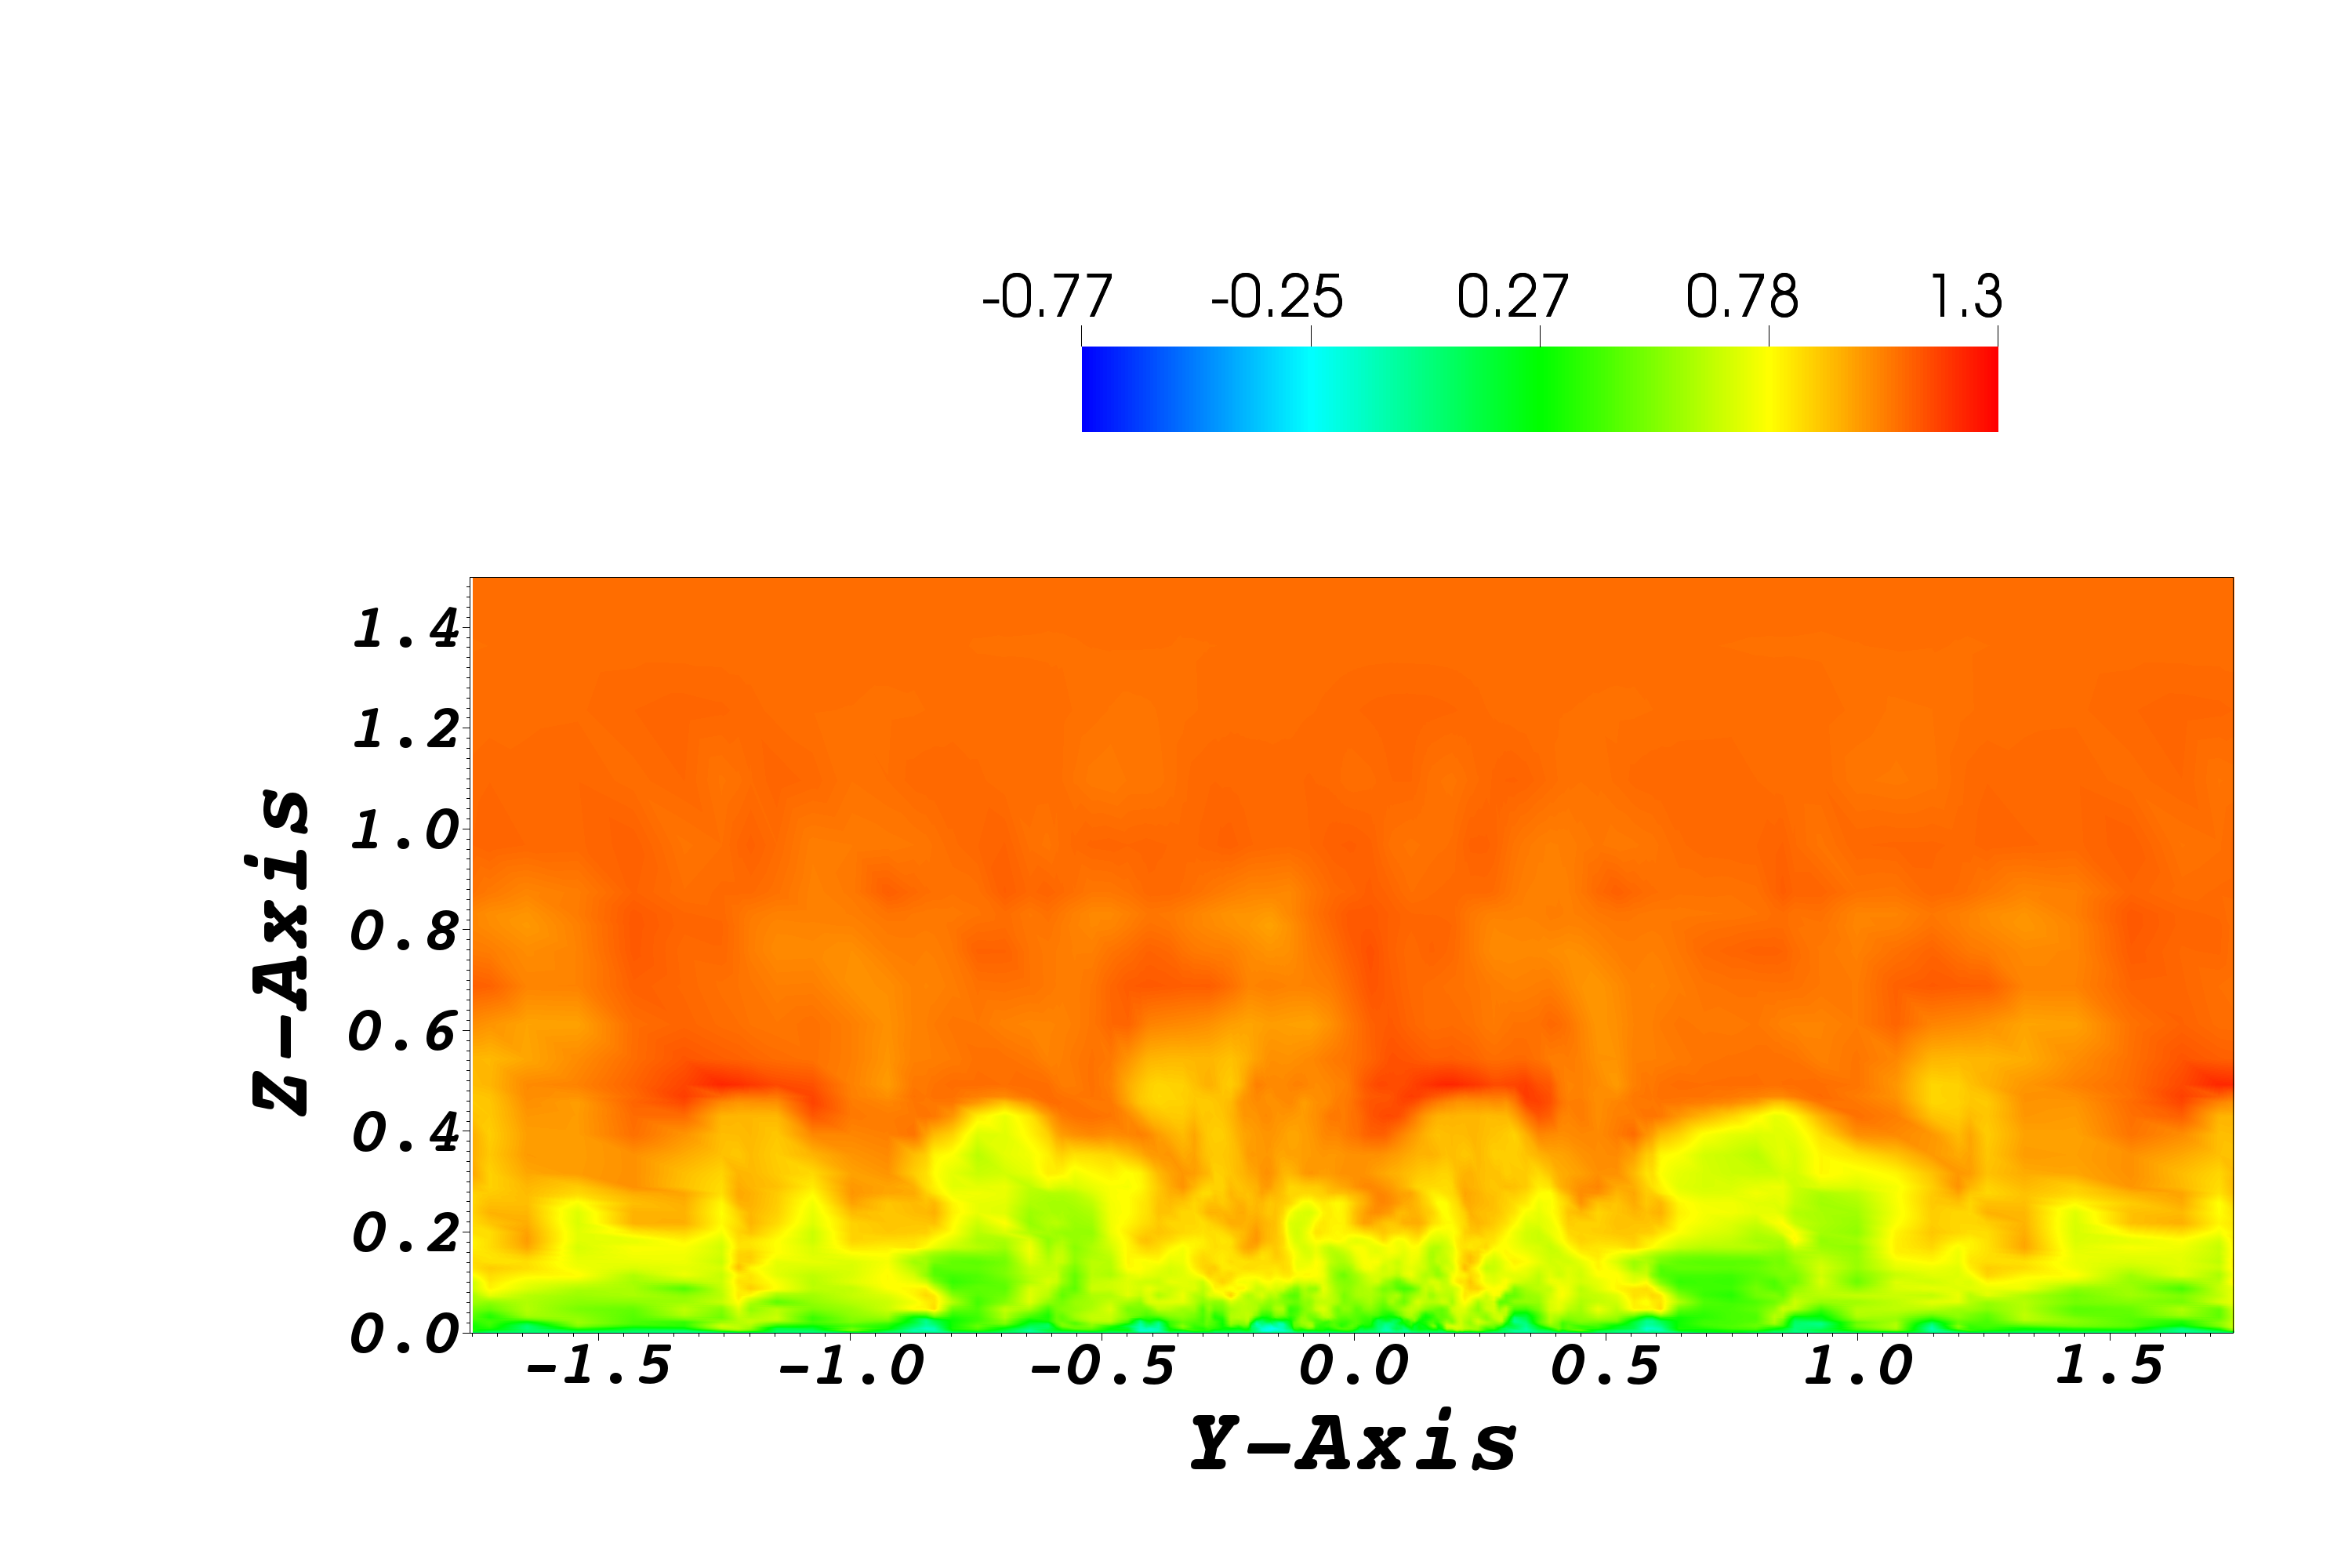
\includegraphics[width=1.0\linewidth]{Figures/inflow_field.png}
\end{minipage}
}
  \caption{The averaged (left) and instantaneous (right) x-velocity on the inflow boundary.}
  \label{fig:inflow}
\end{figure}
%

The simulations in Nek5000 were performed in the following manner; first 6 seconds of initialization of the velocity field in the 
channel, followed by 8 seconds of gas release to initialize the gas-concentration. After assuring that the wind-field was 
correctly created and the released gas had reached the measurement lines furthest from the source the data sampling of 22 seconds 
started.
%
\begin{figure}[h]
	\centering
	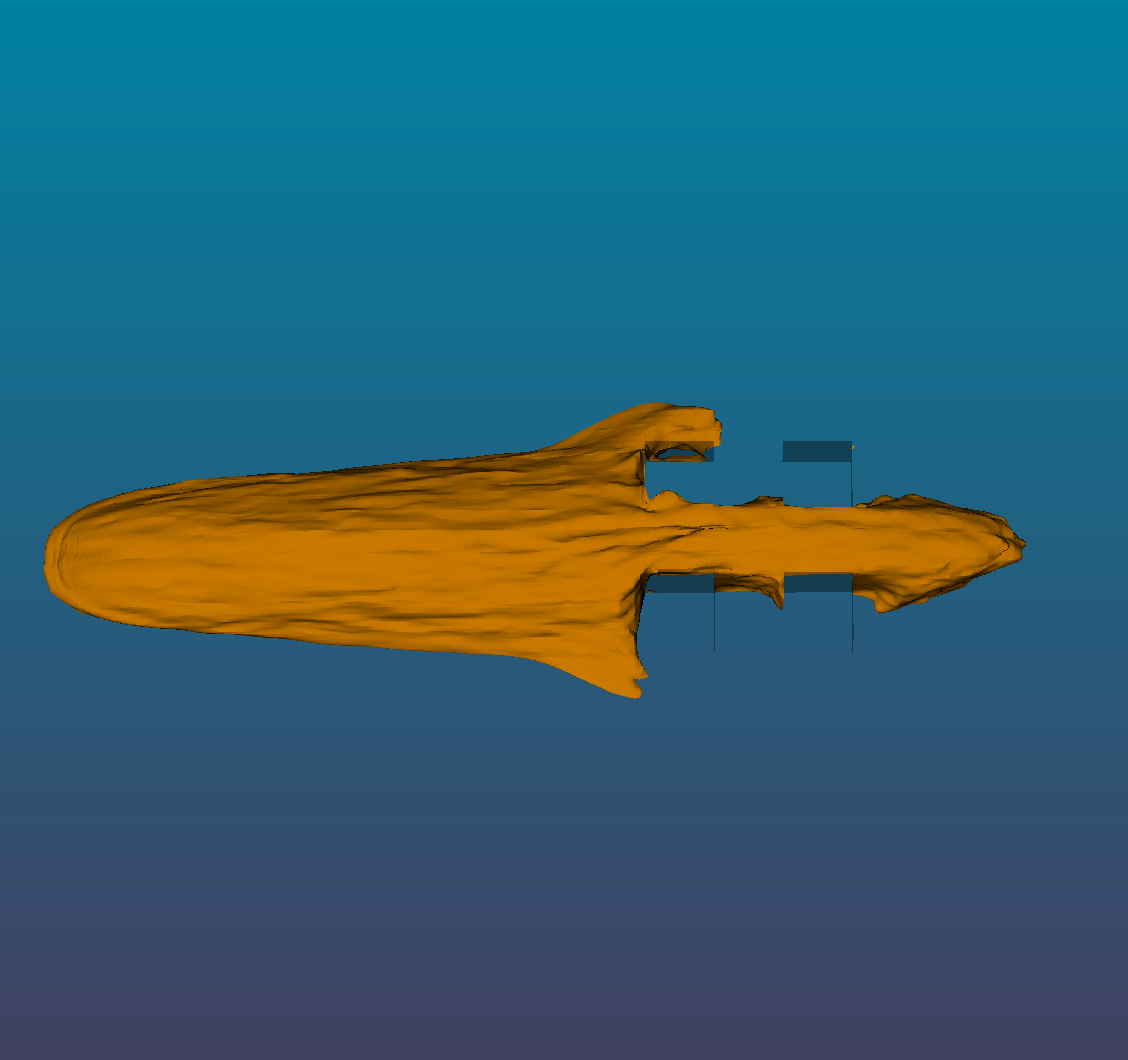
\includegraphics[width=0.6\textwidth]{Figures/plume2.png}
	\caption{An iso-surface of the average concentration with $C=0.03$ 
    after 30 seconds of sampling.}
	\label{fig:plume}
\end{figure}
%

The mesh used in the simulations performed in Nek5000 and the one performed in CDP are 
different, and the resolution in the part of the domain close to the cubes is described 
in~\tref{tab:meshdiff}.
\begin{table}
    \centering
    \begin{tabular}{c| c c c}
        Solver   & $n_x$& $n_y$ & $n_z$ \\ \hline
        CDP      & 28 & 28 & 64 \\ 
        Nek5000  & 22 & 22 & 36 
    \end{tabular}
    \caption{Number of nodes used to represent one cube.}
    \label{tab:meshdiff}
\end{table}

The resolution is better in the simulations done in CDP and especially in 
the $z$-direction. This probably explains some of the differece close to 
$z=0$

\subsection{Results - Gas dispersion} 
This case is a part of a larger project designed to evaluate different solvers 
ability to perform simulations of gas dispersion. The N-S equations are solved using
the $P_NP_N$ formulation with the fractional step method, IOFS with a target Courant number 
equal 2 was enabled to maximize the time step as recommended in~\cite{Nek}. It should be 
mentioned that the stability properties when activating the SGS-model and deactivating the 
filtering was greatly reduced. This effect is captured in~\fref{fig:maxvel} that shows how 
the Smagorinsky model does not damp spurious velocity modes in the same degree as the filter. 
%
\begin{figure}[h]
	\centering
	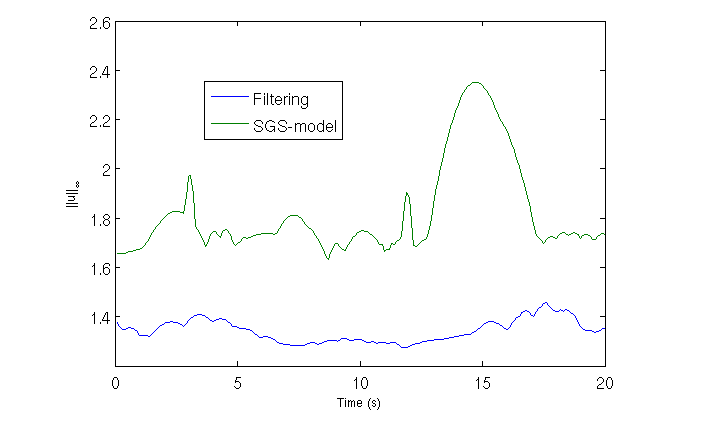
\includegraphics[width=0.6\textwidth]{Figures/maxvel.png}
    \caption{$||\mathbf{u}||_{\infty}$ as a function of time, the green line represents the 
simulation with the dynamic Smagorinsky SGS-model and the blue line represents the filtering 
with $\alpha = 0.05$ and a quadratic decay on the last 3 modes.}
	\label{fig:maxvel}
\end{figure}
%
%
%\begin{figure}[h]
	%\centering
	%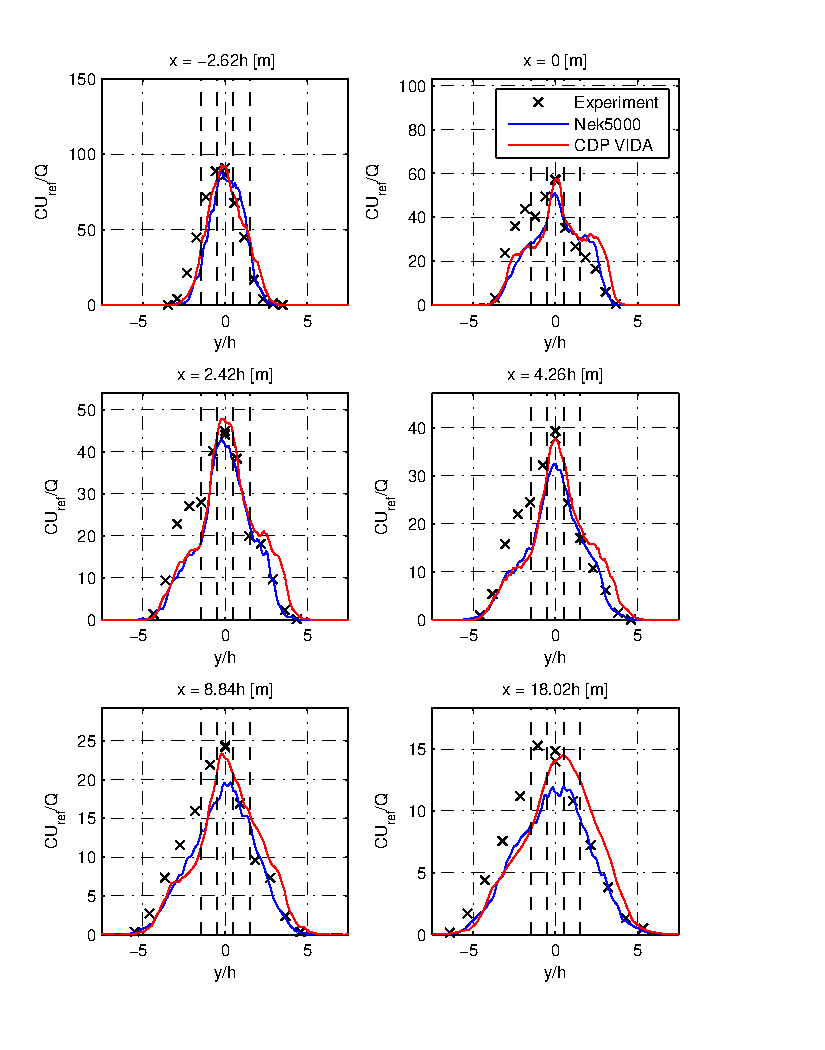
\includegraphics[width=0.8\textwidth]{Figures/NekcH.pdf}
	%\caption{Time-averaged concentration with a sample time of $18.00$ s at $z/H = 0.025$ plotted horizontally and scaled 
	%with the free-stream velocity and emission rate. Compared against wind tunnel data.
%Two dashed lines on either side of the centerline represent the canyon.}
	%\label{fig:cHfilter}
%\end{figure}
%
%
%\begin{figure}[h]
	%\centerline{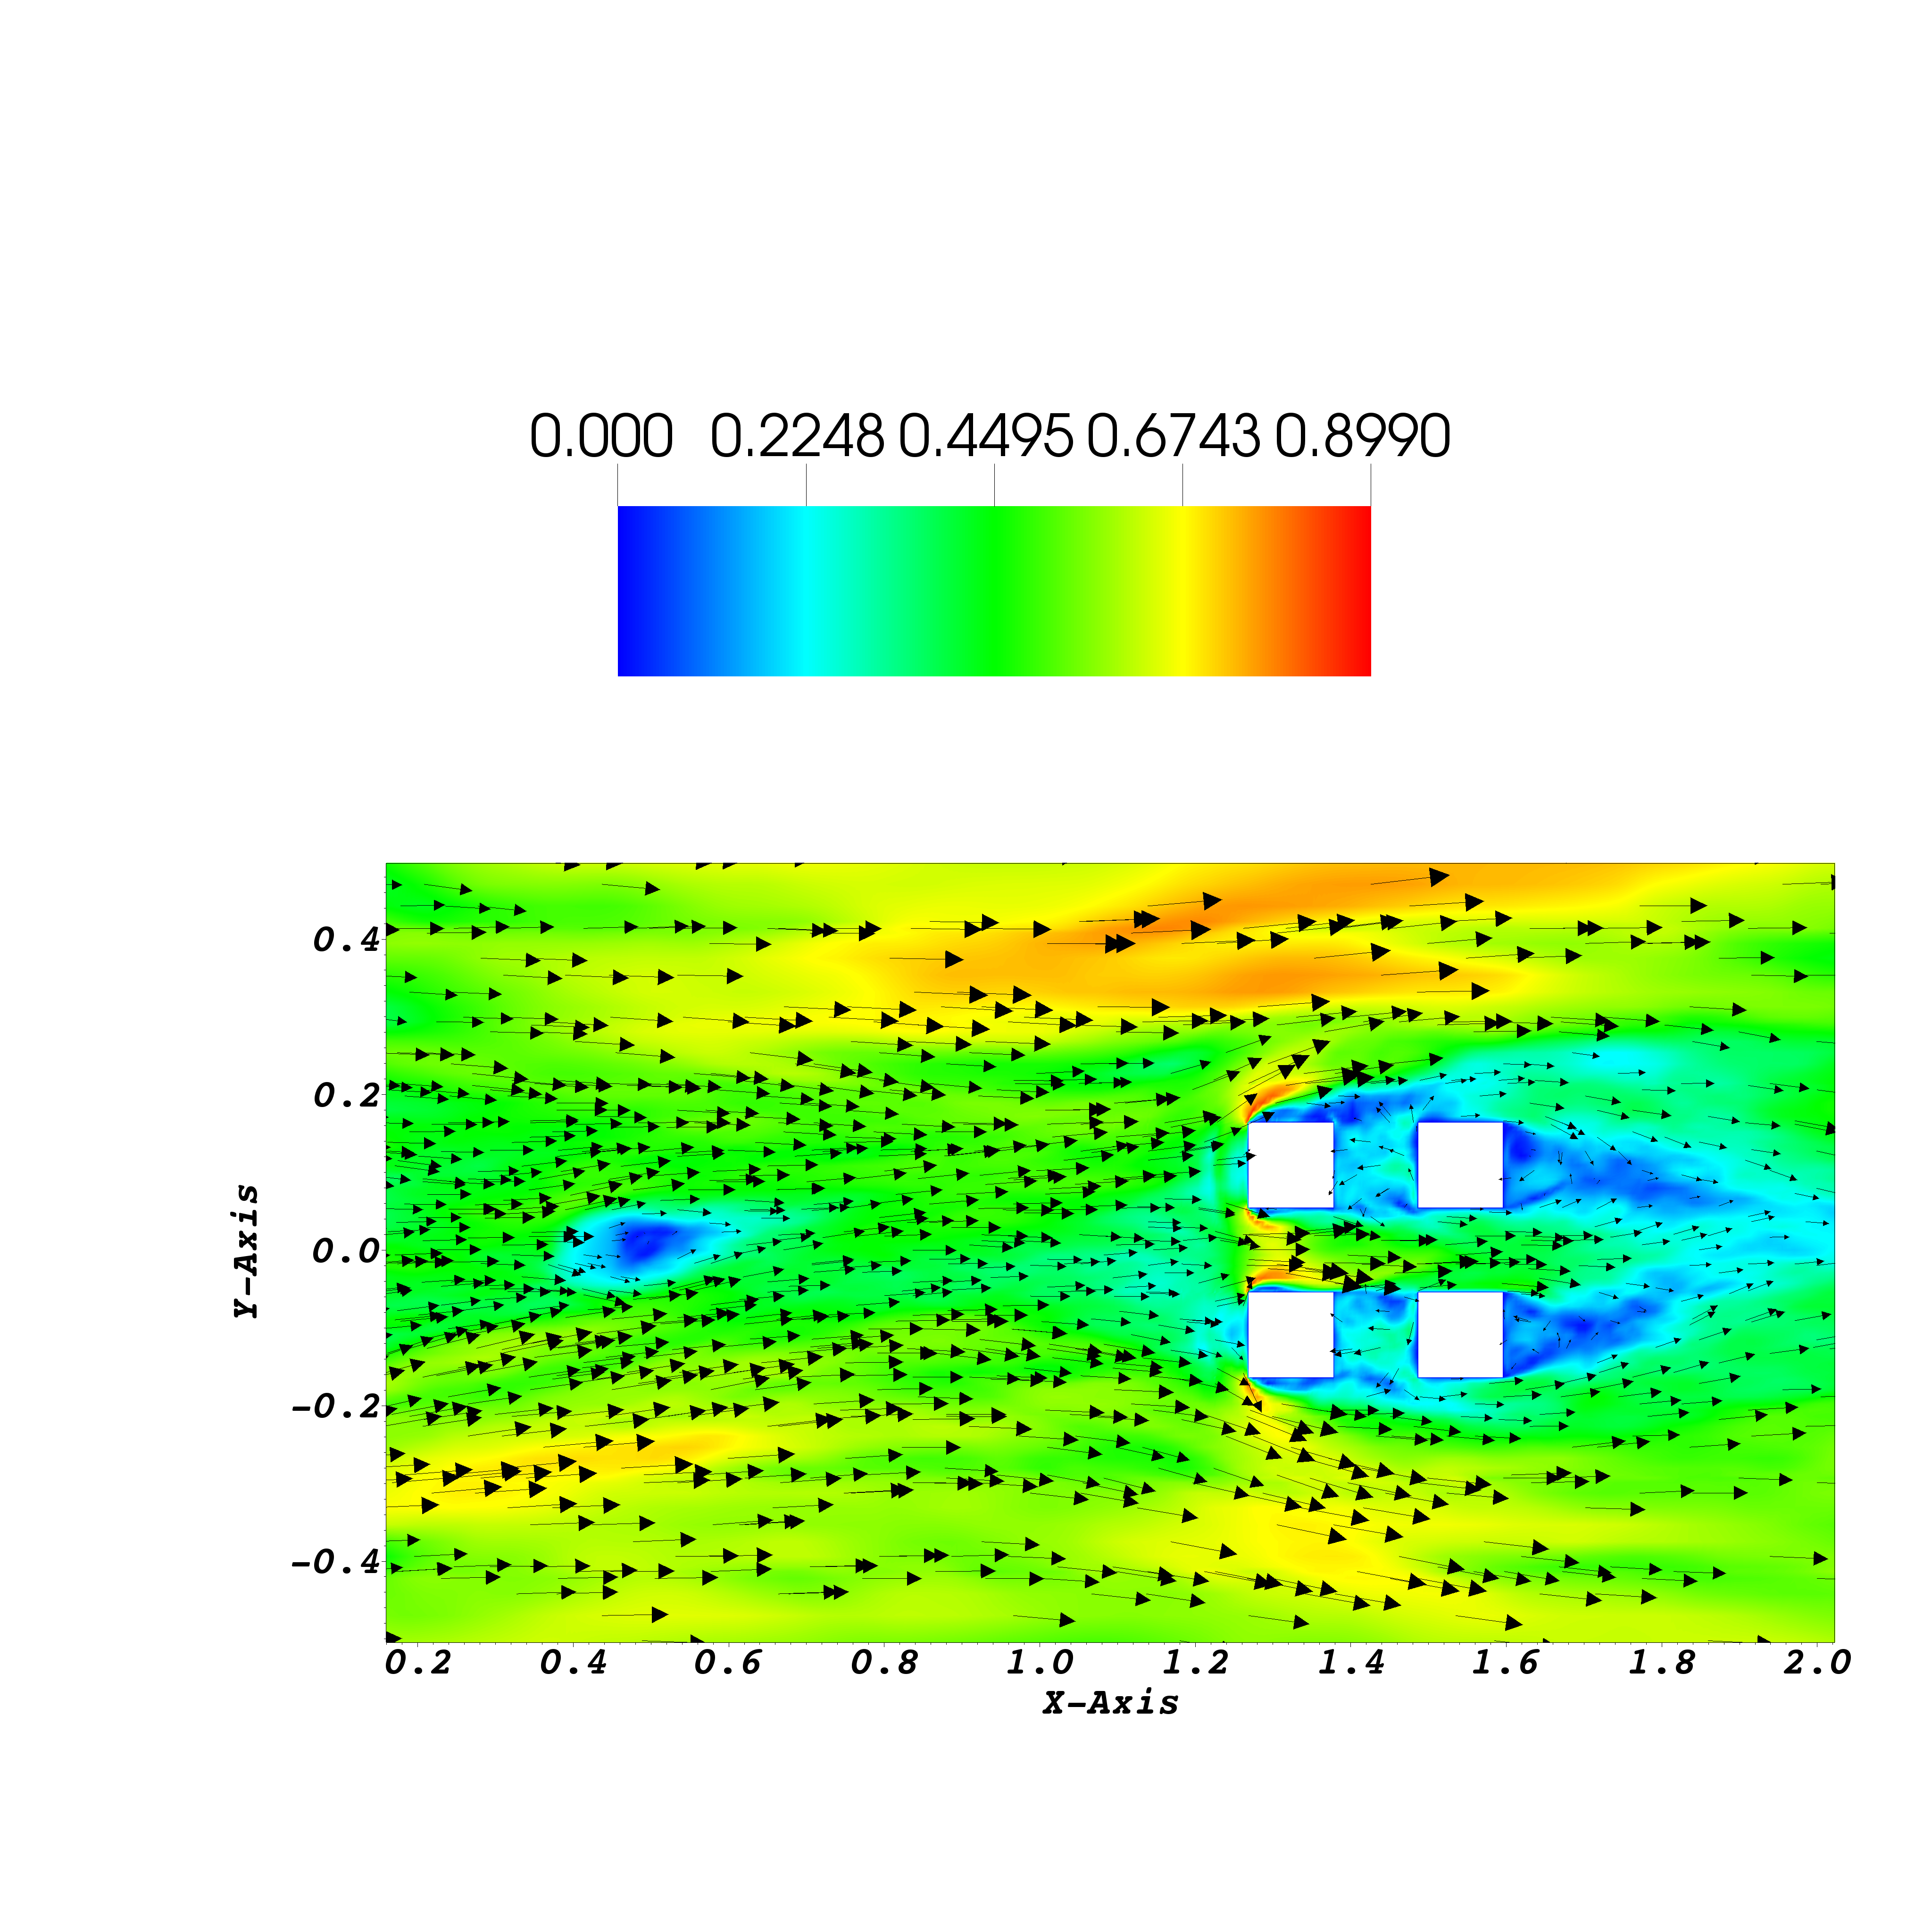
\includegraphics[width=0.8\textwidth]{Figures/vel_field.png}}
	%\caption{velocity field for $z= 0.02$m, around the source and the cubes.}
	%\label{fig:vel_field}
%\end{figure}
%

%\colorbox{green}{redo these simulation in case they were started to early.}
%
%\begin{figure}[h]
	%\centering
	%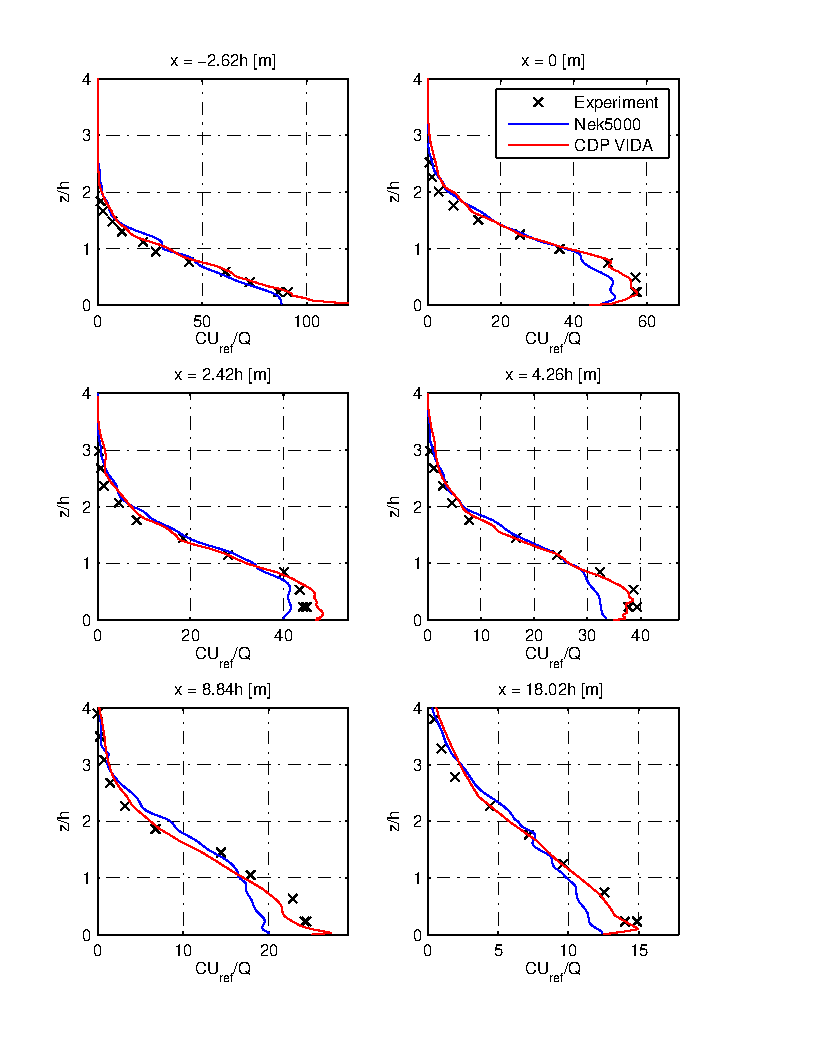
\includegraphics[width=0.8\textwidth]{Figures/NekcV.pdf}
	%\caption{Time-averaged concentration with a sample time of $18.00$ s at $y = 0$ plotted
    %vertically and scaled 
	%with the free-stream velocity and emission rate. Compared against wind tunnel data.
%Two dashed lines on either side of the centerline represent the canyon.}
	%\label{fig:cVfilter}
%\end{figure}
%
%
%\begin{figure}[h]
	%\centering
	%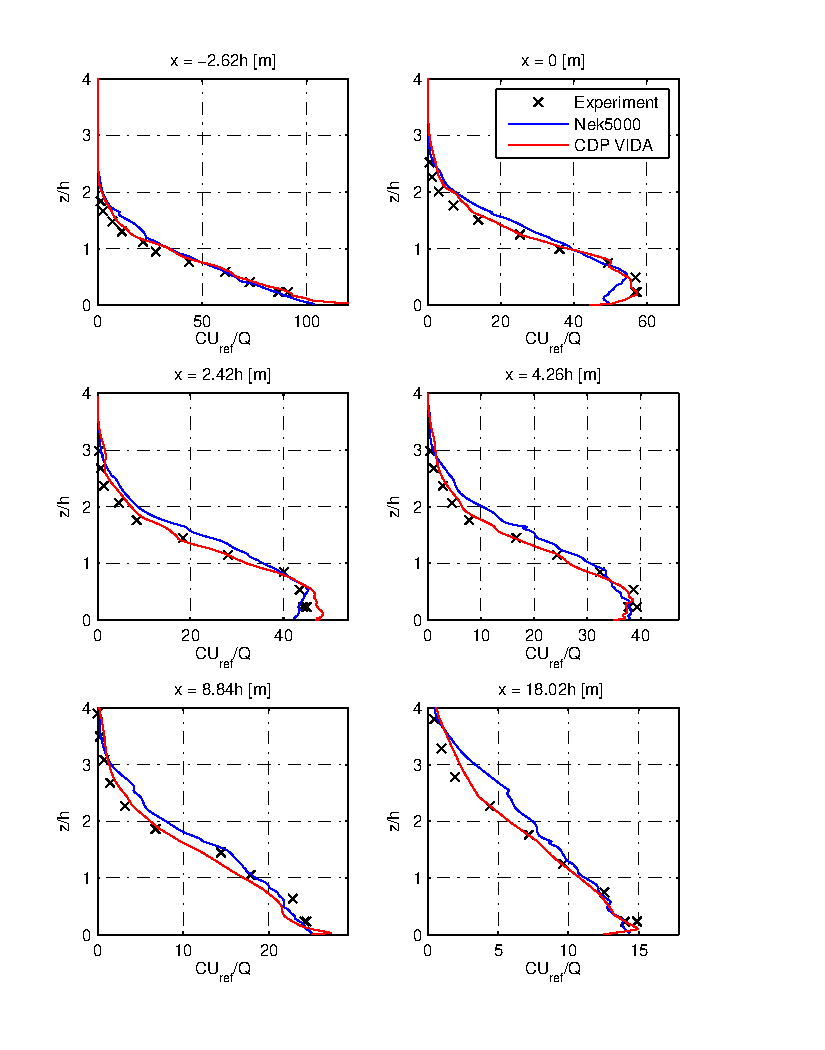
\includegraphics[width=0.8\textwidth]{Figures/Nek_smag_cV.pdf}
	%\caption{Time-averaged concentration with a sample time of $22.00$ s at $y = 0$ plotted
    %vertically and scaled 
	%with the free-stream velocity and emission rate. Compared against wind tunnel data.
%Two dashed lines on either side of the centerline represent the canyon.}
	%\label{fig:cVsmag}
%\end{figure}
%
%
%\begin{figure}[h]
	%\centering
	%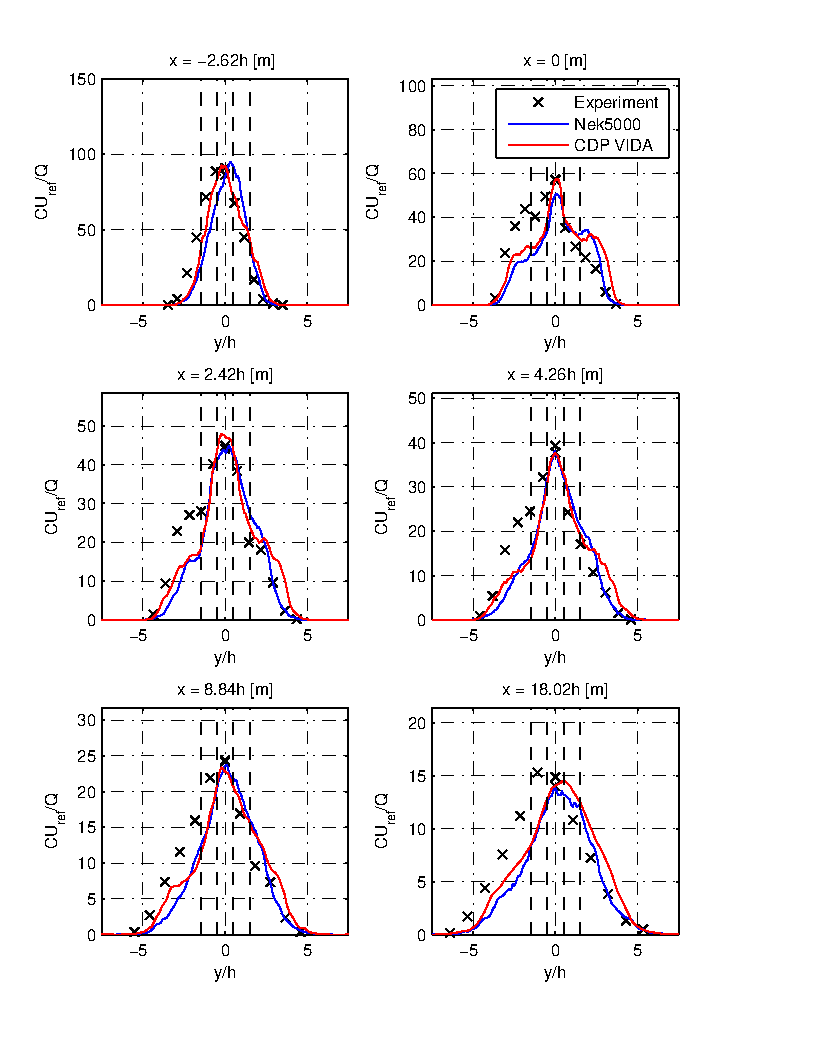
\includegraphics[width=0.8\textwidth]{Figures/Nek_smag_cH.pdf}
	%\caption{Time-averaged concentration with a sample time of $22.00$ s at $y = 0$ plotted
    %vertically and scaled 
	%with the free-stream velocity and emission rate. Compared against wind tunnel data.
%Two dashed lines on either side of the centerline represent the canyon.}
	%\label{fig:cVsmag}
%\end{figure}
%
\newpage
\begin{figure}[h]
    \centering
    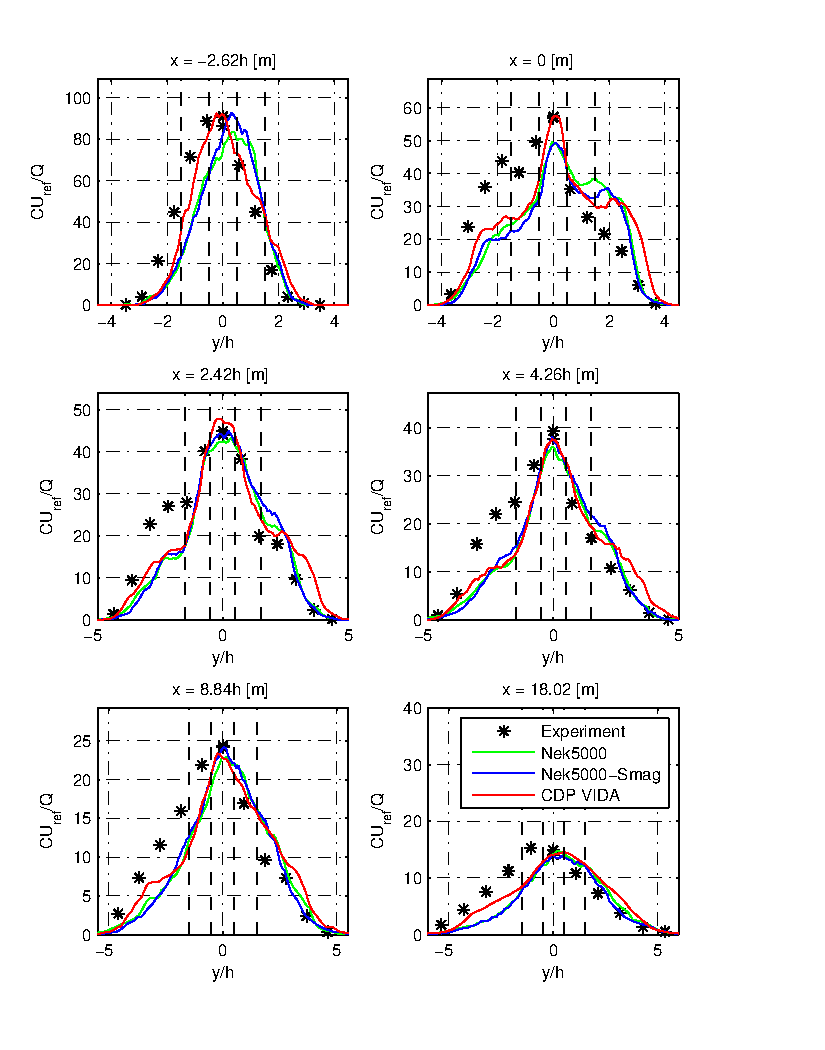
\includegraphics[width=0.8\textwidth]{Figures/NekcH_all.pdf}
    \caption{Time-averaged concentration with a sample time of $22.00$ s at $y = 0$ plotted
    vertically and scaled 
    with the free-stream velocity and emission rate. Compared against wind tunnel data.
Two dashed lines on either side of the centerline represent the canyon.}
    \label{fig:cHall}
\end{figure}

\fref{fig:cHall} shows the scaled concentration along the dotted lines in~\fref{fig:layout}. 
According to this figure Nek5000 does indeed capture the important features of the mean concentration.
At the two first measurement lines the results are slightly skewed to the right, this is to some degree 
also the case for the CDP simulations but not for the experiment. A possible explanation could be that 
the inflow condition favours one of the sides of the domain, or simply that the sampling time is not 
sufficiently long. 
%Along the second measurement line which is placed in the middle of the 4 cubes Nek5000 
%estimates a concentration peak lower than both the reference solutions.  

The results also indicate that the difference between the SGS-model and the filtering
is not that large,
if anything the SGS-model shows a tendency to estimate higher concentration peaks.
In particular the first plot indicates a significant difference.
An important difference between the filtering and the SGS-model is 
that the filter works based on the current state of the flow 
whereas the amount of diffusion added by the SGS-model is mostly decided
by the previous states of the flow.
This could lead to either too much or too little smoothening locally.

\newpage
\begin{figure}[h]
    \centering
    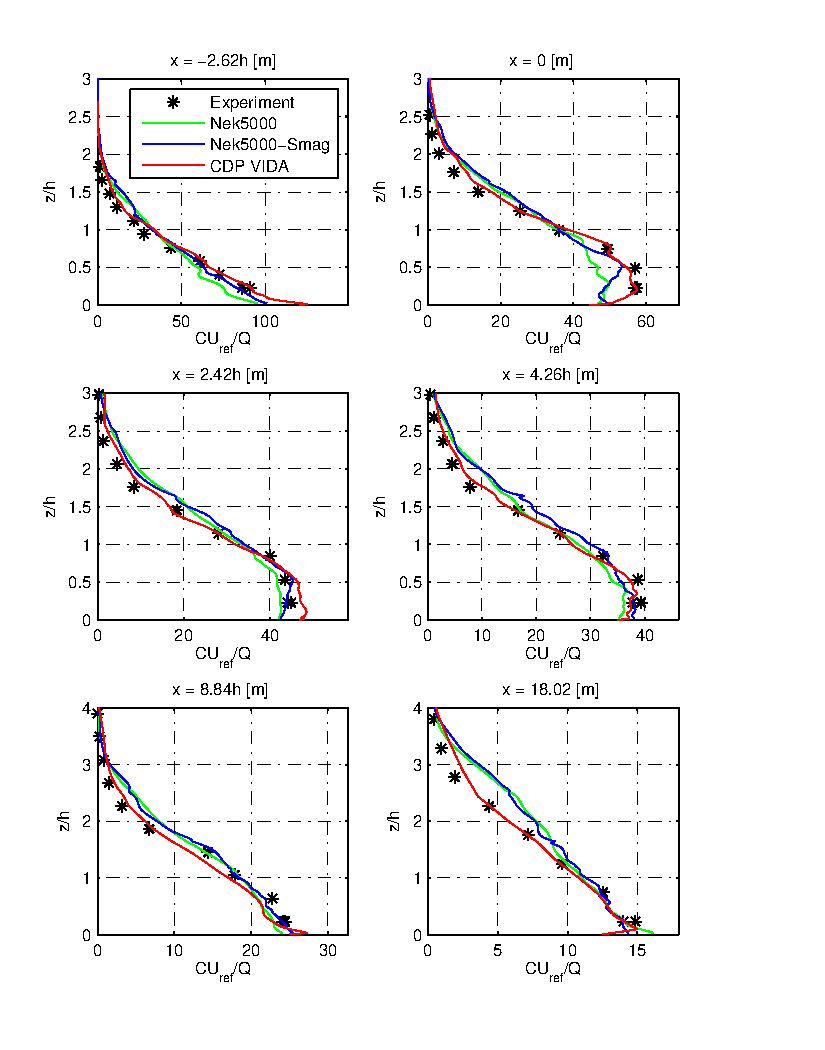
\includegraphics[width=0.8\textwidth]{Figures/NekcV_all.pdf}
    \caption{Time-averaged concentration with a sample time of $22.00$ s at $y = 0$ plotted
    vertically and scaled 
    with the free-stream velocity and emission rate. Compared against wind tunnel data.
Two dashed lines on either side of the centerline represent the canyon.}
    \label{fig:cVall}
\end{figure}
The concentration along the vertical measurement lines is plotted in \fref{fig:cVall} and overall 
Nek5000 provides good results according to the reference solutions. The largest difference is found close 
to the wall right in the middle of the cubes. In particular the simulation with filtering 
underestimates the concentration in this domain. The resolution of the mesh used for the 
Nek5000 simulations in this area is notably worse than for the CDP-simulations.
And in the middle of the cubes neither one of the filter or the Dynamic Smagorinsky model
are able to correct this.
The $P_NP_N$ formulation is known to produce splitting errors of significant sizes 
close to the wall, and could play an important role in this part of the domain.


%\begin{figure}[h]
    %\centering
    %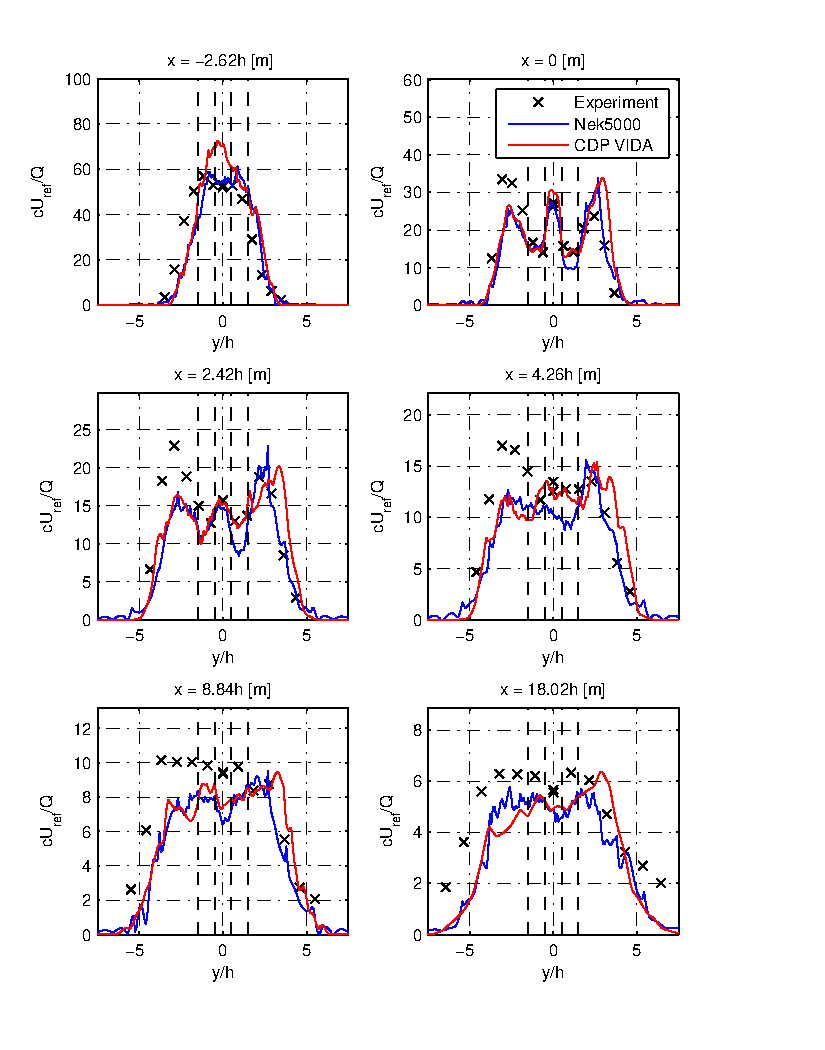
\includegraphics[width=0.8\textwidth]{Figures/Nek_smag_cfluctH.pdf}
    %\caption{Time-averaged concentration with a sample time of $22.00$ s at $y = 0$ plotted
    %vertically and scaled 
    %with the free-stream velocity and emission rate. Compared against wind tunnel data.
%Two dashed lines on either side of the centerline represent the canyon.}
    %\label{fig:cVsmag}
%\end{figure}


\section{Case 2: Drag and lift on a cylinder}
A standard benchmark case for flow solvers is presented in~\cite{benchmark}. 
The case is to calculate the drag and lift coefficients on a cylinder in a rectangular channel.
The setup for the domain and boundary conditions are given in \fref{fig:cylinder}.
The constants applied in the description of the geometry and the coefficient scales are listed 
in table \tref{tab:case2consts}.
%
\begin{table}[h]
    \centering
    \begin{tabular}{c l l}
     Constant & Value & Property \\ \hline
    $H$ & $0.41\text{m}$ & Width and height for the channel \\
    $D$ & $0.1\text{m}$ & Diameter of the cylinder and length scale \\
    $U$ & $0.2\text{m/s}$ & Velocity scale \\
    $\nu$ &  $ 10^{-3}\text{m$^2$/s}$ & Kinematic viscosity of the fluid \\
    $Re$ & $20$ & Reynolds number \\ 
    \end{tabular}
    \caption{Constants for case 2}
    \label{tab:case2consts}
\end{table}
%
Finding the drag and lift coefficient requires a calculation of the velocity field around the cylinder
which is done by solving the unsteady N-S equations until a steady flow is reached. This implies that the
spatial accuracy will dominate the error and one would expect great results in Nek5000 
due to its spectral convergence rate.

The flow is laminar with Reynolds number $Re=20$ so all the 
challenges arising when dealing with turbulent flow does not come to play in this case. 
%
\begin{figure}[h]
    \centering
    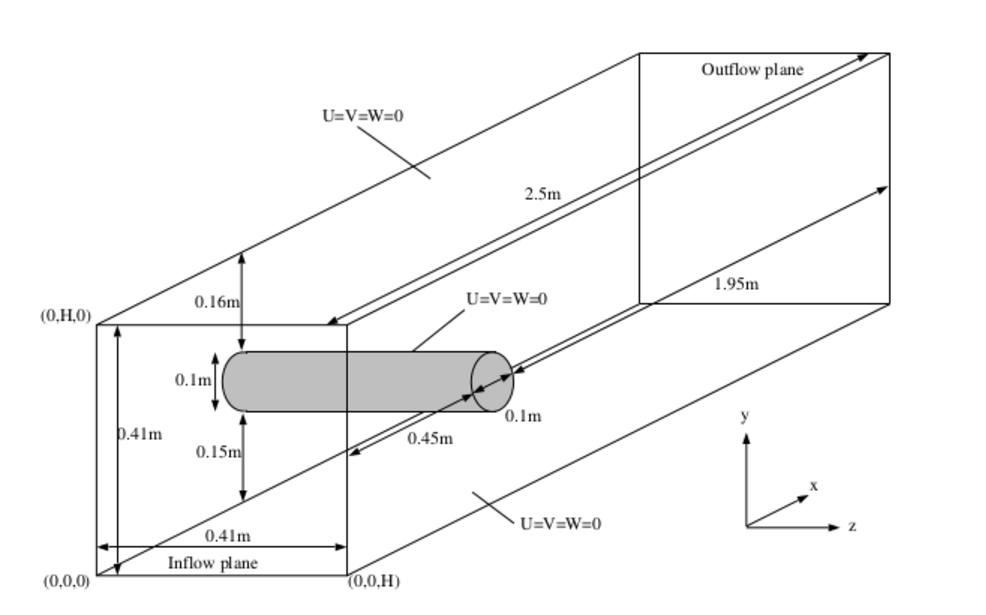
\includegraphics[width = 1.0\textwidth]{Figures/cylinder.pdf}
    \caption{Computational domain and boundary conditions.}
    \label{fig:cylinder}
\end{figure}
%
The drag and lift forces on a surface $S$ are given as 
%
\begin{align}
    F_D = \int_{S}(\rho \nu \frac{\partial v_t}{\partial n}n_y-pn_x)dS, \qquad
    F_L = -\int_{S}(\rho \nu \frac{\partial v_t}{\partial n}n_x+pn_y)dS.
    \label{eq:dragnlift}
\end{align}
%
$v_t$ is the tangential velocity, $\mathbf{n}=[n_x,n_y,0]$ is the unit vector normal to the surface $S$ 
and the tangent velocity vector is defined as $\mathbf{t} = [n_y,-n_x,0]$.
 
Surface integrals in Nek5000 are solved numerically, $\int_S f dS = \sum f_i A_i$, where $f$ is some function and $A_i$ is the area corresponding
to the nodal value $f_i$. $A_i$ corresponds to a two dimensional mass matrix in Nek5000 available for all elements.

The coefficients corresponding to these forces known as the drag and lift coefficients 
are given by the formulas 
\begin{align}
    c_D = \frac{2F_D}{\rho U^2 D H}
    \qquad , \qquad
    c_L = \frac{2F_L}{\rho U^2 D H}.
    \label{eq:dragnliftcoeffs}
\end{align}


Nek5000 provides functions for calculating lift and drag on any user-specified object.
The function is called \verb|drag_calc(scale)|, with the input parameter 
defined by the user, for this case \verb|scale| $=2/(\rho U^2DH)$.  
Apart from this the function \verb|set_obj()| has to be modified in order to create an object 
that consists of pointers to all the faces on the cylinder.
%Let $x,y$ be points in the computational domain, $x_c,y_c$ be the coordinates to the 
%center line in the cylinder and $0<tol\ll1$ be some user defined tolerance. The faces that belong to the cylinder can then be found by 
%looping over all elements and their faces evaluating $\epsilon = \sqrt{(x-x_c)^2+(y-y_c)}$.
%If $\epsilon < tol$ for an entire face then this face is known to 
%belong to the cylinder and is added to the object. Nek also allows the user to specify multiple objects 
%assigning the faces of interest to object 1, object 2 etc. The geometry and mesh 
%for this case was generated in ICEM, and the total number of elements are 2070. 
%For the final calculation polynomial degree $P = 11$ was applied leading to a 
%total of $N = 2755170$.
%
\begin{figure}[h]
    \centering
    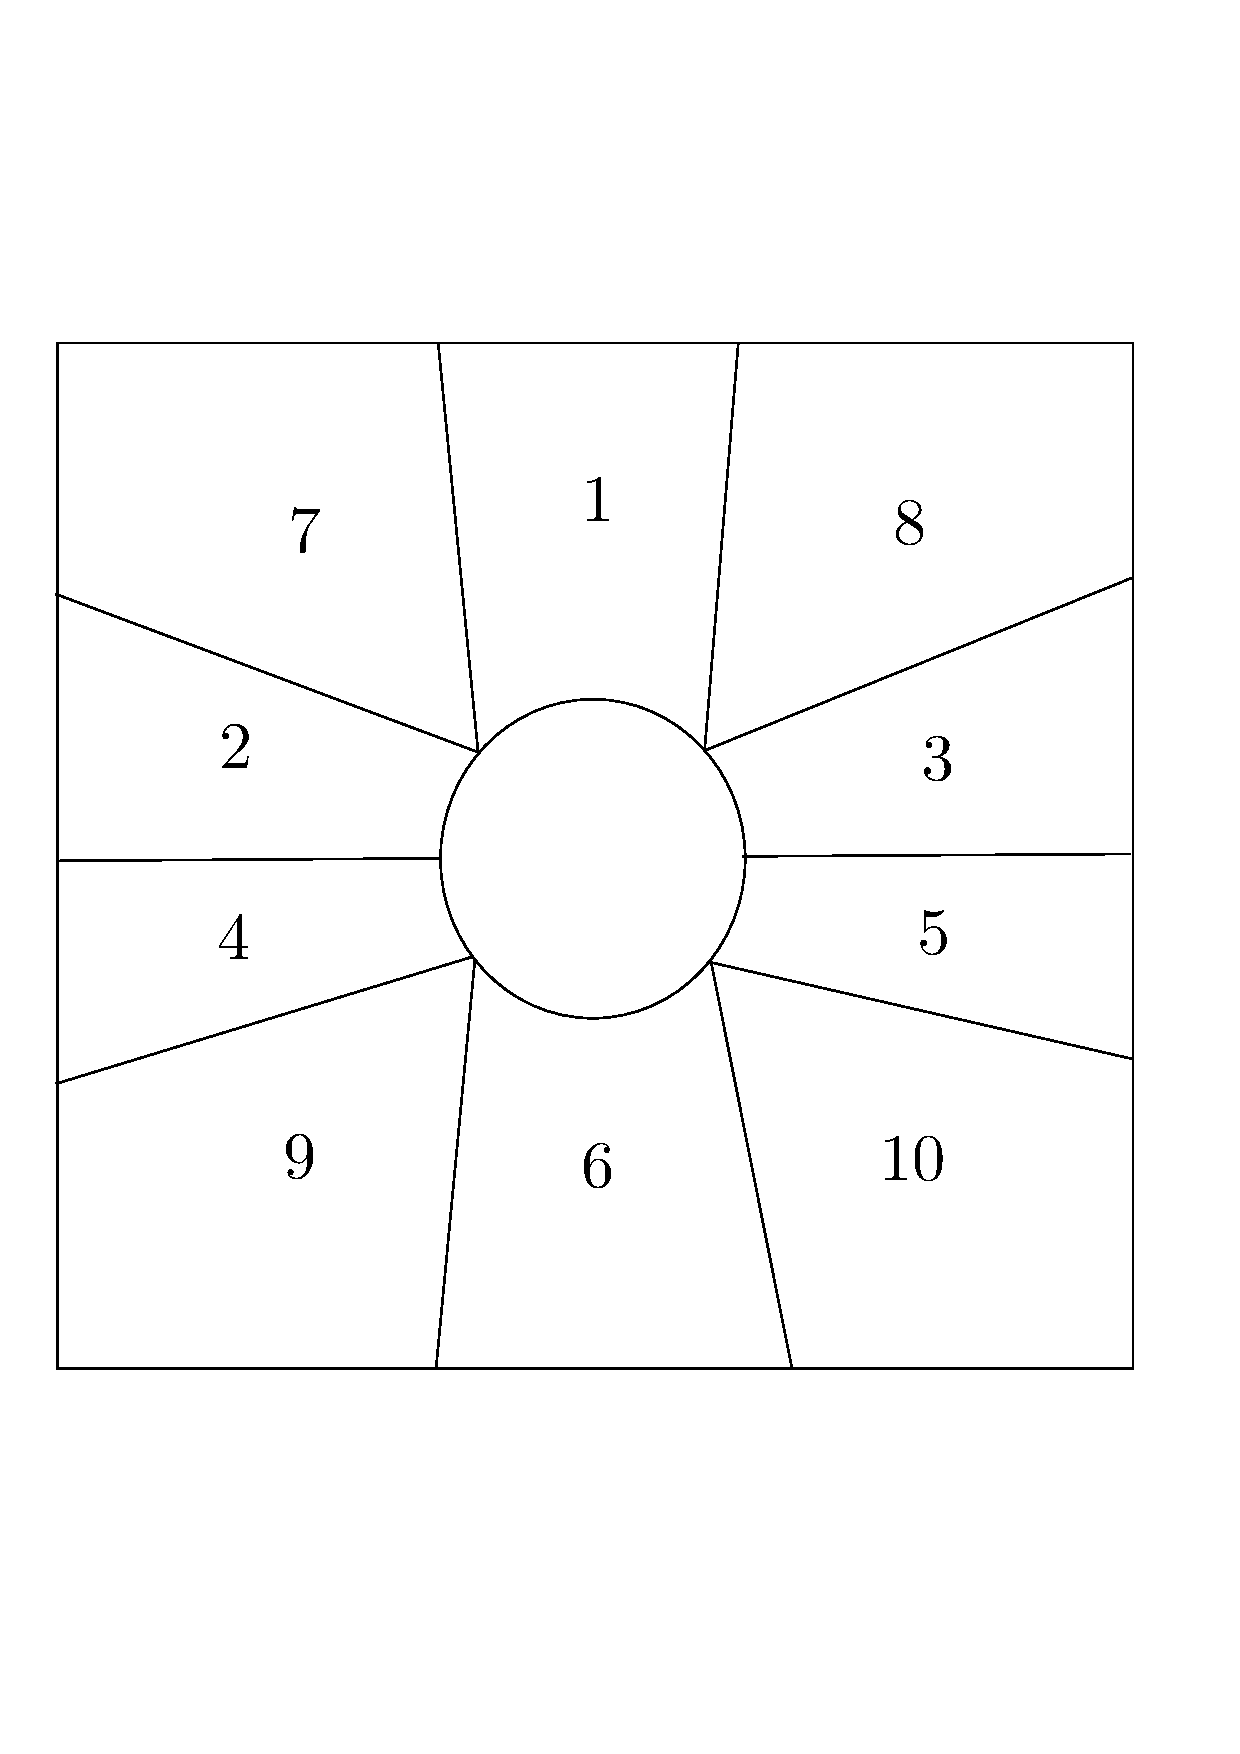
\includegraphics[width = 0.3\textwidth]{Figures/cyl_elem.pdf}
    \caption{Initial mesh around cylinder.}
    \label{fig:cyl_elem}
\end{figure}
%
The mesh around the cylinder is illustrated in \fref{fig:cyl_elem}.
Initially this case was solved using a second degree polynomial to describe the circle segments
corresponding to each element. However with the new routine implemented as described 
in~\cref{xyzarc} the circle segments could be represented with the same order as 
the polynomials used for the velocity space. The importance of the error resulting 
from the second degree approximation of the circle segments is presented in \cref{results}.
%Note that these elements was split in three, in order to obtain 
%a finer mesh in the region of interest. Of the elements numbered in~\fref{fig:cyl_elem}
%only the first six contains edges on the cylinder.Hence the second order polynomials 
%describing the curved edges describe approximately $\Theta = 360^{\circ}/(6\cdot 3) = 20^{\circ}$
%of the complete circle. 

An additional test that is performed on this case is how different settings in Nek5000 will affect the estimation of the drag and lift coefficients.
Perhaps most curious is whether the $P_NP_N$ or $P_NP_{N-2}$ formulation is applied. Note that the pressure in the latter formulation is 
not defined on the boundary of the cylinder and does therefore need to be extrapolated onto the surface in order for the integral to be 
calculated. On the other side is the splitting scheme implied by the $P_NP_N$ forces the erroneous boundary condition on the pressure.
%
\subsection{Results - benchmark comparison}
The effect of the algorithm explained in \cref{xyzarc} is
illustrated by solving a laminar flow test problem. 
The solution is compared with previously benchmark computations performed by a number of 
contributors~\cite{benchmark}. 

The results are presented in \tref{tab:testcase}, and they confirm that the treatment of the geometry is 
essential, both coefficients are computed with significantly better accuracy. 
%
\begin{table}[h]
\centering
\begin{tabular}{l l c c c c}
		\toprule
		\# of Cells & Software & $c_D$ & $c_L$ & \%\textbf{Err} $c_D$ &\%\textbf{Err} $c_L$ \\ \midrule 
		2755170& Nek5000 (mid) & 6.18349 & 0.008939 & 0.030 & 4.19 \\ 
		2755170& Nek5000 (arc) & 6.18498 & 0.009413 & 0.006 & 0.13 \\
		3145728 & CFX 		 & 6.18287 & 0.009387 & 0.04 &0.15 \\
		3145728 & OF	     & 6.18931 & 0.00973 & 0.06 &3.5 \\
		3145728 & FEATFLOW   & 6.18465 & 0.009397 & 0.01 &0.05 \\
		\bottomrule	
	\end{tabular}
	\caption{Results for the drag and lift coefficients with reference values 
	$c_D = 6.18533$ and $c_L = 0.009401$. $p=11$ for the simulations in Nek5000.}
\label{tab:testcase}
\end{table}
%
Compared with the results from the other softwares applied in~\cite{benchmark} Nek5000 performs 
just as well or better in most cases. It should be mentioned that the division of the grid is created
in a different manner for Nek5000 so the comparison is not as direct as it may seem from the table.

\subsection{Results - internal adjustments }
As discussed in \cref{nek} there are many adjustments available in Nek5000. 
In order to enlighten the actual effect on the results, several different settings were 
investigated for this case and the results are presented in \tref{tab:perf}. 
The spectral convergence is also confirmed in \fref{fig:liftconv} by calculating the 
lift coefficient error for increasing polynomial degree. 
%
\begin{figure}[h]
	\centerline{
        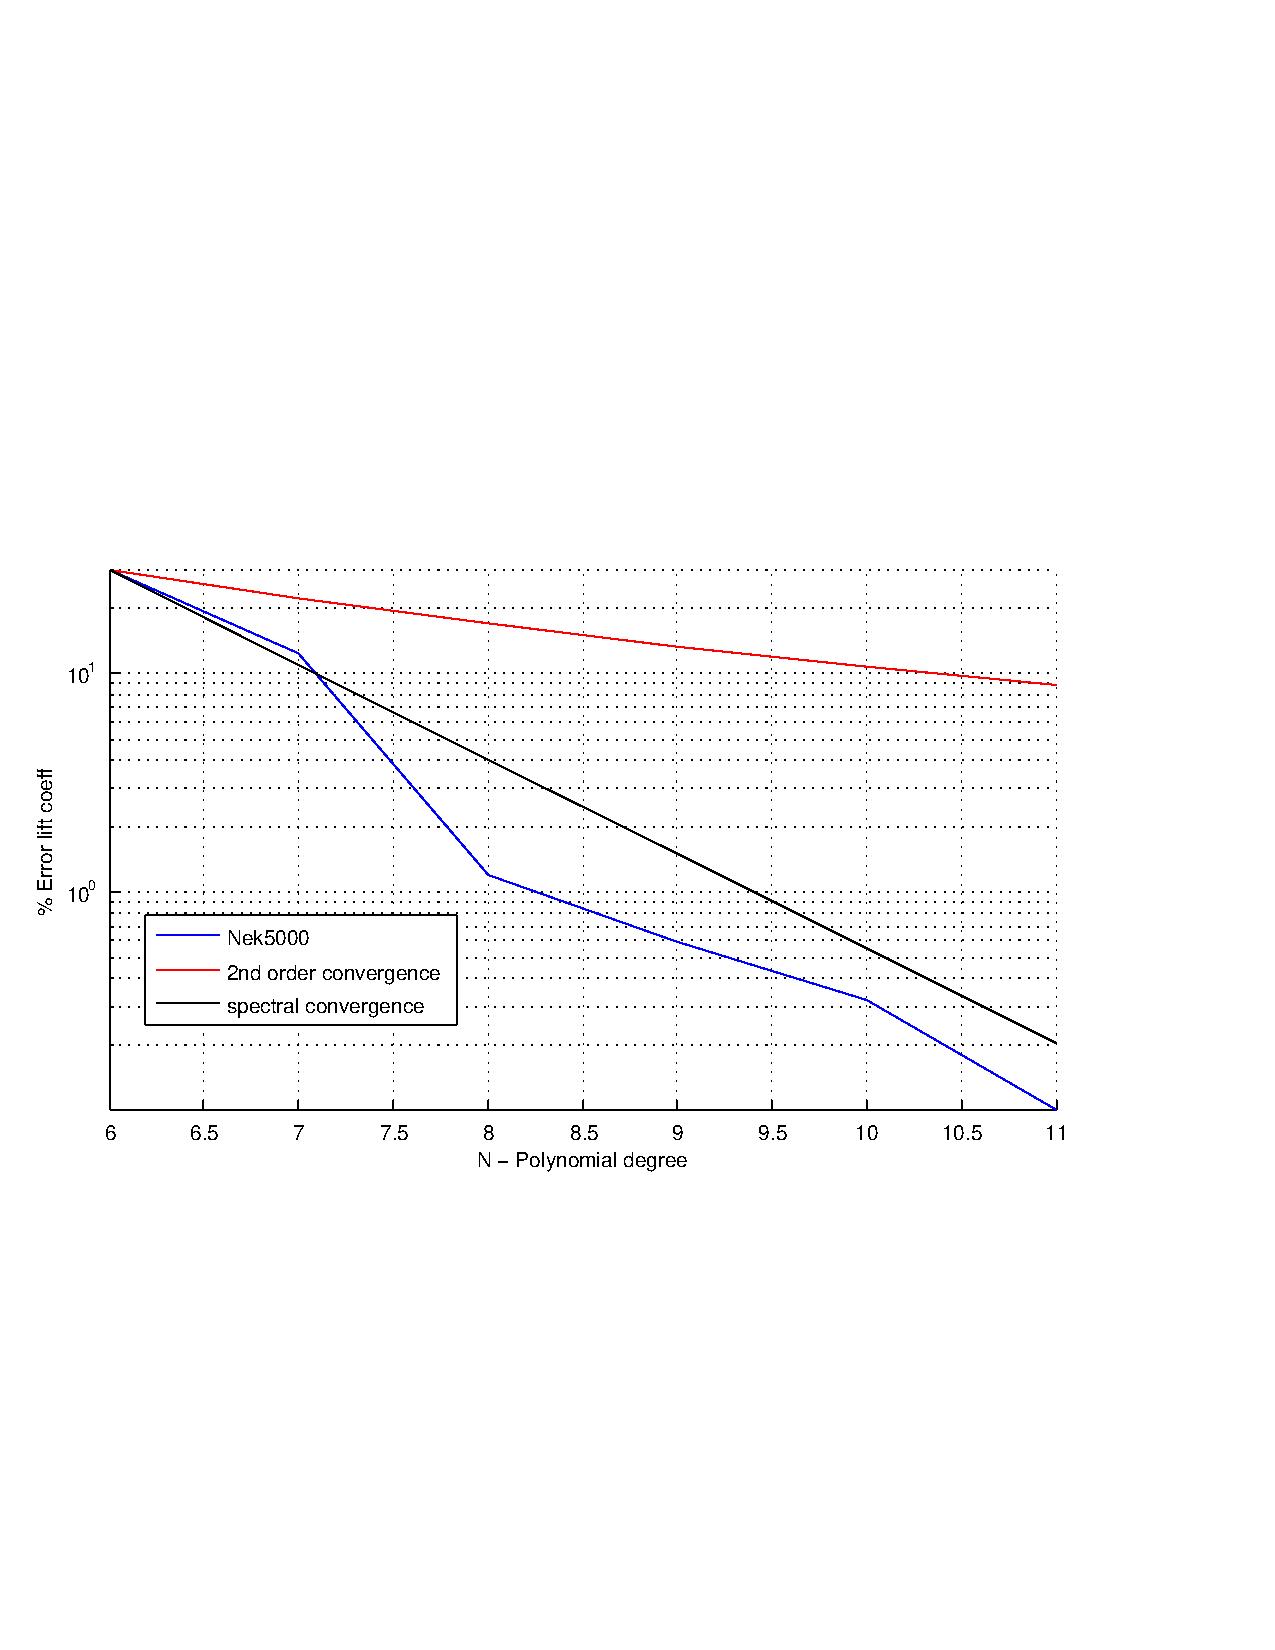
\includegraphics[trim=0.5cm 7cm 0.5cm 7cm, width=0.8\textwidth]{Figures/lift_coef4.pdf}}
	\caption{The logarithm of the error plotted against the polynomial degree. All results 
        are with $P_NP_{N-2}$ and dealiasing, and they are solved without using the 
    characteristic scheme or any filtering. A line illustrating a second order convergence is 
    plotted to illustrate the convergence rate.}
	\label{fig:liftconv}
\end{figure}
%

The setting that has the biggest impact on the result is the $P_NP_N$ scheme which clearly performs 
worse than the others. This is as expected since the discrete splitting is known to converge faster
for steady state flows. Notice however that by reducing the time-step the effect of the algebraic splitting
greatly reduces and achieves results of similar order as the discrete splitting.
Use of the IOFS method also has a negative effect on the accuracy,
this is also as expected because of the stability-accuracy trade-off for this method.
Remember that this scheme allows a much higher time step. The filtering is the least significant change
which confirms the analytical results from \eref{eq:filterenergy}. 
%
\begin{table}[h]
    \centering
    \begin{tabular}{c | c c c c c | c c }
         & \multicolumn{5}{|c|}{Settings} & \multicolumn{2}{|c}{\% Error} \\\hline
         \# & $\Delta t$ & ifsplit & Dealiasing & IOFS & Filter & $c_D$ & $c_L$ \\  \hline 
         1 & 6e-4& No & Yes& No & No & 0.005 & 0.10\\
         2 & 6e-4& No & Yes& No & Yes& 0.005 & 0.43\\
         3 & 6e-4& No & Yes& Yes& No & 0.005 & 0.18\\
         4 & 6e-4& No & No & No & No & 0.005 & 0.03\\
         5 & 6e-4& Yes& Yes& No & No & 0.013 & 2.35\\
         6 & 4.5e-4& Yes& Yes& No & No & 0.002 & 0.01\\
         7 & 3e-4& Yes& Yes& No & No & 0.002 & 0.01\\
    \end{tabular}
    %\begin{tabular}{c | c c c c | c c | c c c}
         %& \multicolumn{4}{|c|}{Settings} & \multicolumn{2}{|c|}{\% Error} & \multicolumn{3}{|c}{Data} \\\hline
         %\#  & ifsplit & Dealiasing & IOFS & Filter & $c_D$ & $c_L$ & DT & CFL & T/Tstep \\ \hline 
         %1 & F & T & F & F & 0.005 & 0.102 & 1e-04 & 2.03 & 2.1e-02 \\
         %2 & T & T & F & F & 0.013 & 2.349 & 1e-04 & 2.03 & 2.1e-02 \\
         %3 & F & T & F & T & 0.005 & 0.431 & 1e-04 & 2.03 & 2.1e-02 \\
         %4 & F & T & T & F & 0.005 & 0.179 & 1e-04 & 2.03 & 2.1e-02 \\
         %5 & F & F & F & F & NaN   & NaN   & 1e-04 & 2.03 & 2.1e-02 \\
    %\end{tabular}
    \caption{Test of solver settings in Nek5000.}
    \label{tab:perf}
\end{table}
%

Be aware that these results are obtained from a laminar test case and does not in any way 
suggest any optimal adjustment for Nek5000. An important example of this is the fact that 
deactivating de-aliasing yields better results. For a coarser mesh or a more turbulent flow 
this would not be the case, and that the result is actually better is probably due to 
the accuracy, which are very close to the accuracy given by the reference solution. 
The resuslts do however give an indication to the general effect of these settings that 
are worth noticing.

%----------------------------------------------------------------------------------------
\section{Discussion and Conclusion}
\colorbox{green}{How did Nek5000 perform overall, user-friendly ?,correctness,speed etc.}

